% \begin{figure*}[]

% % \subfloat{%
% %   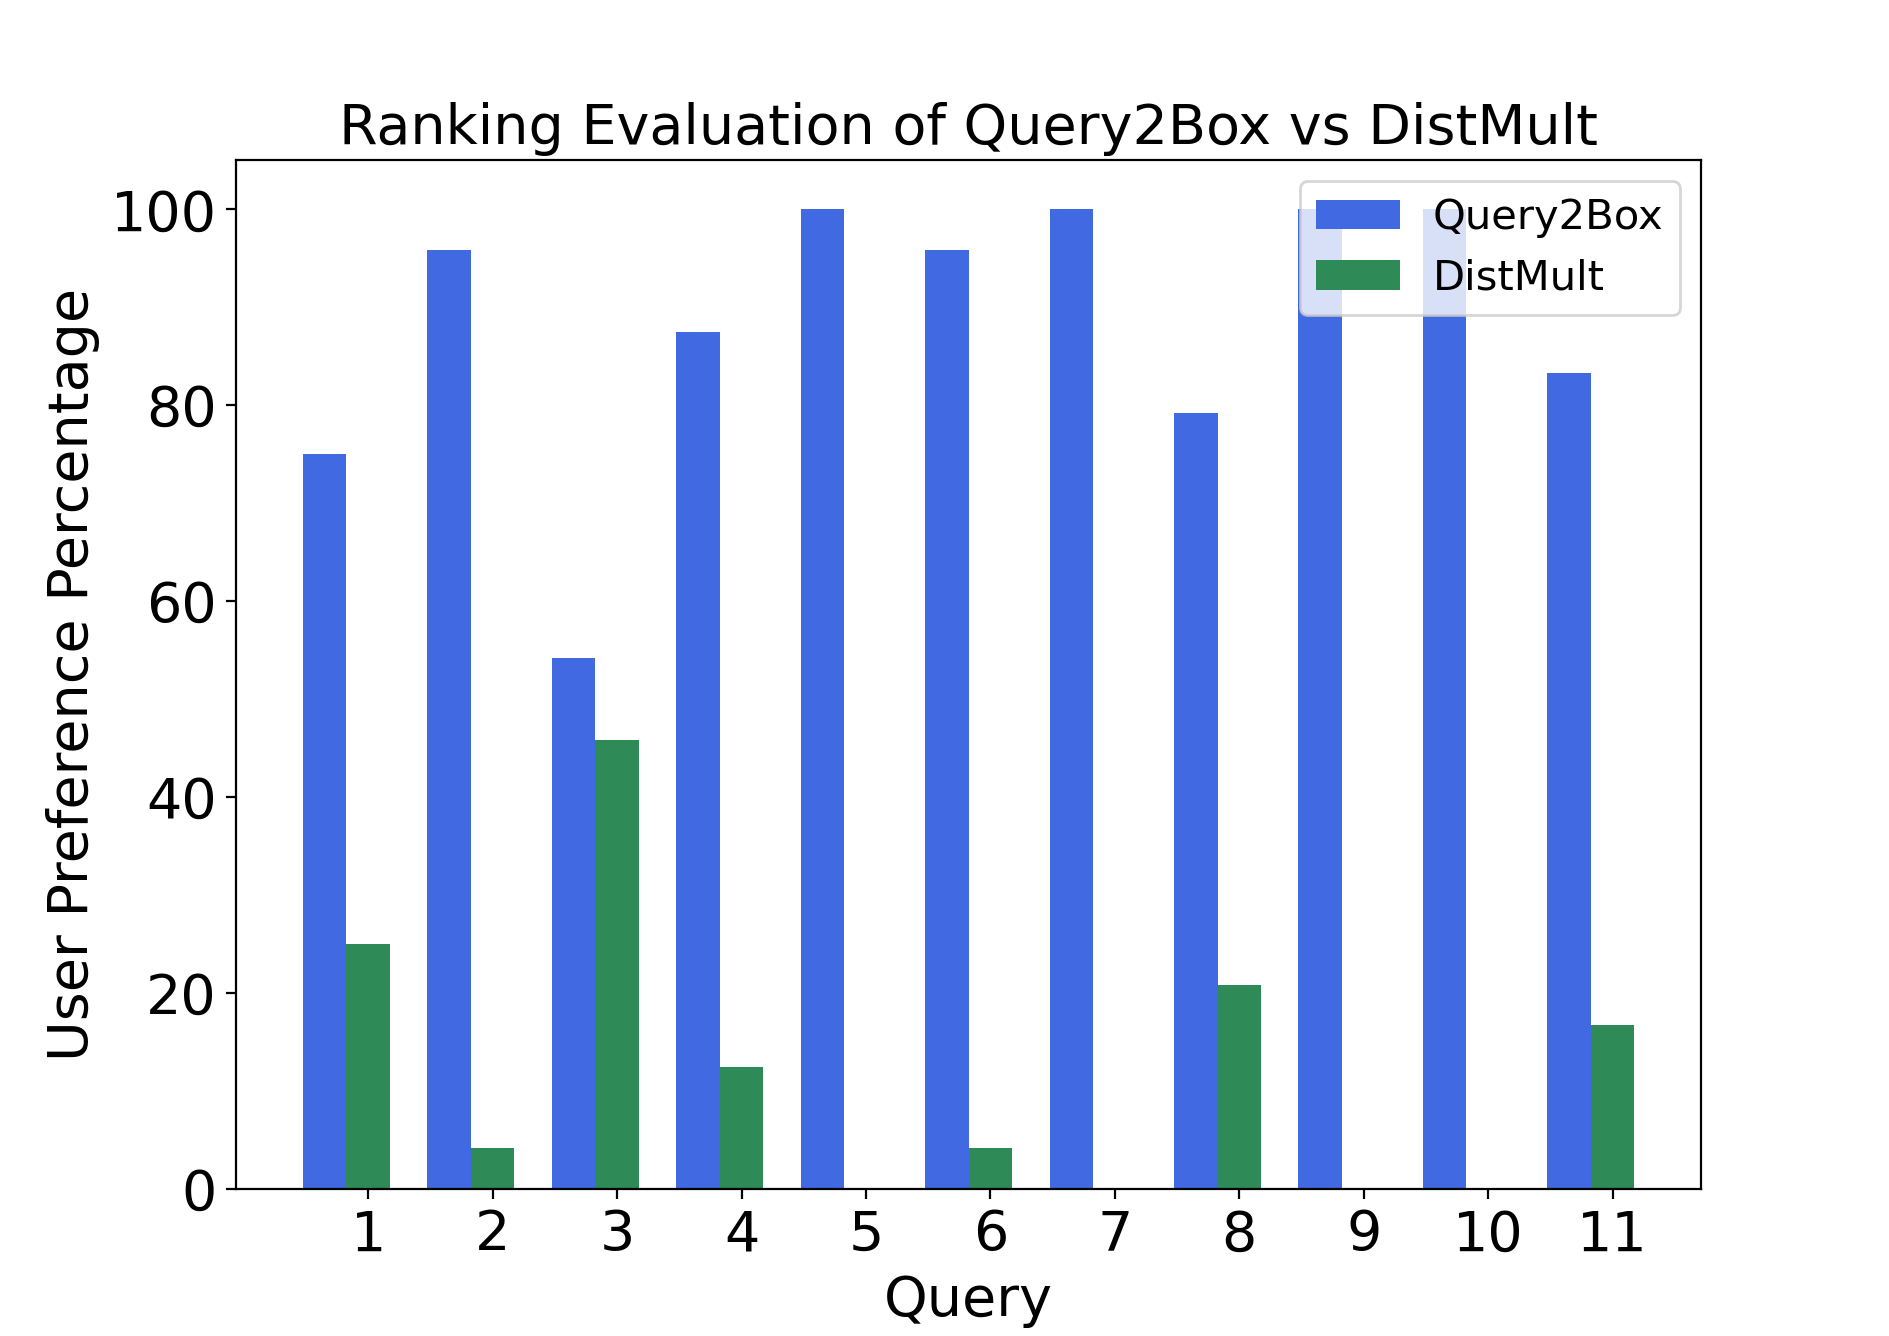
\includegraphics[clip,width=0.75\columnwidth]{submissions/Ali2023/figures/q2b_distmult.png}%
% % }
% \subfloat{%
%   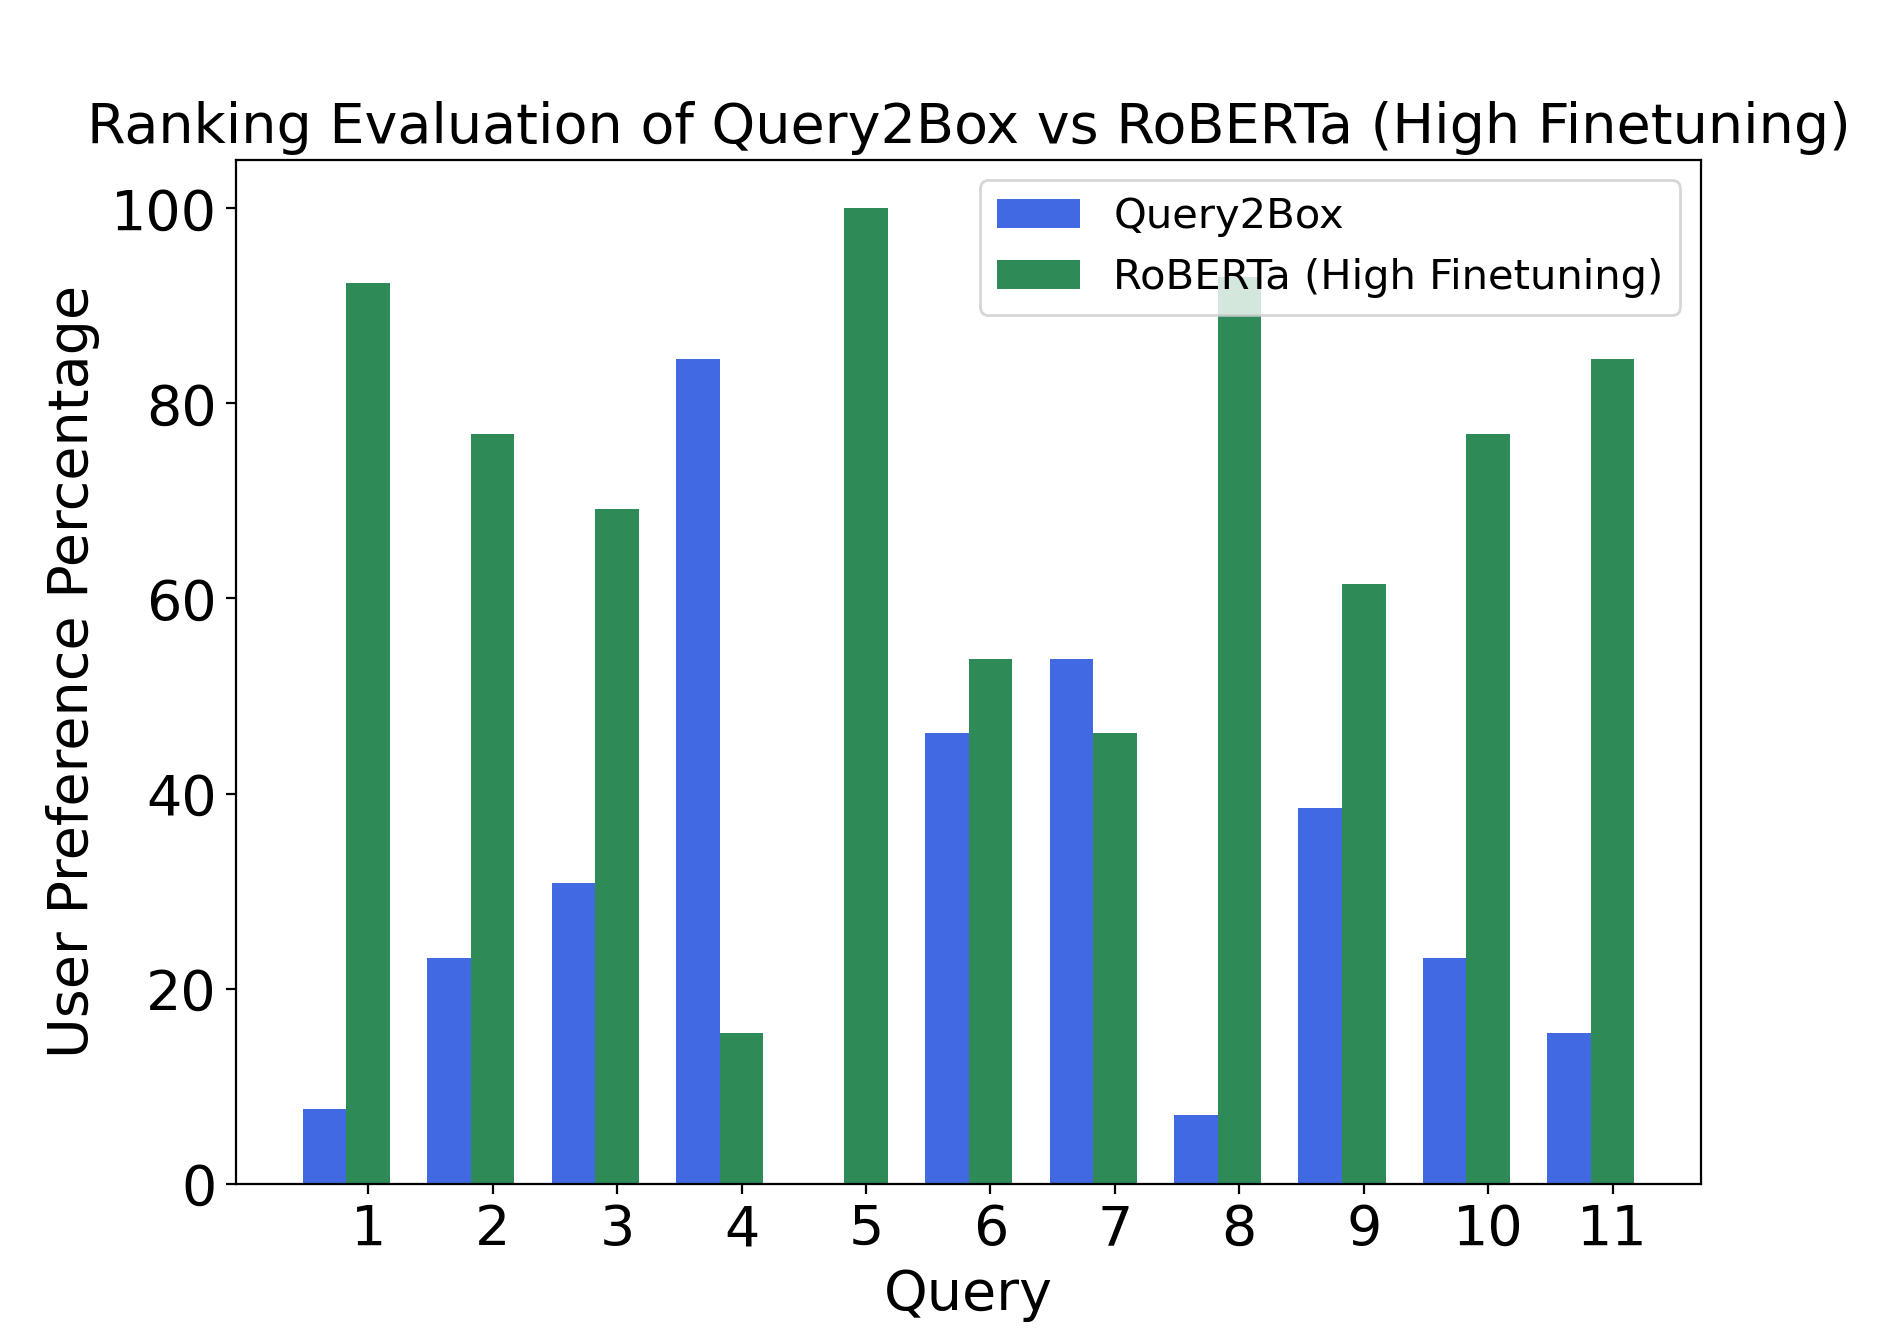
\includegraphics[clip,width=0.65\columnwidth]{submissions/Ali2023/figures/q2b_r1.png}%
% }
% ~
% \subfloat{%
%   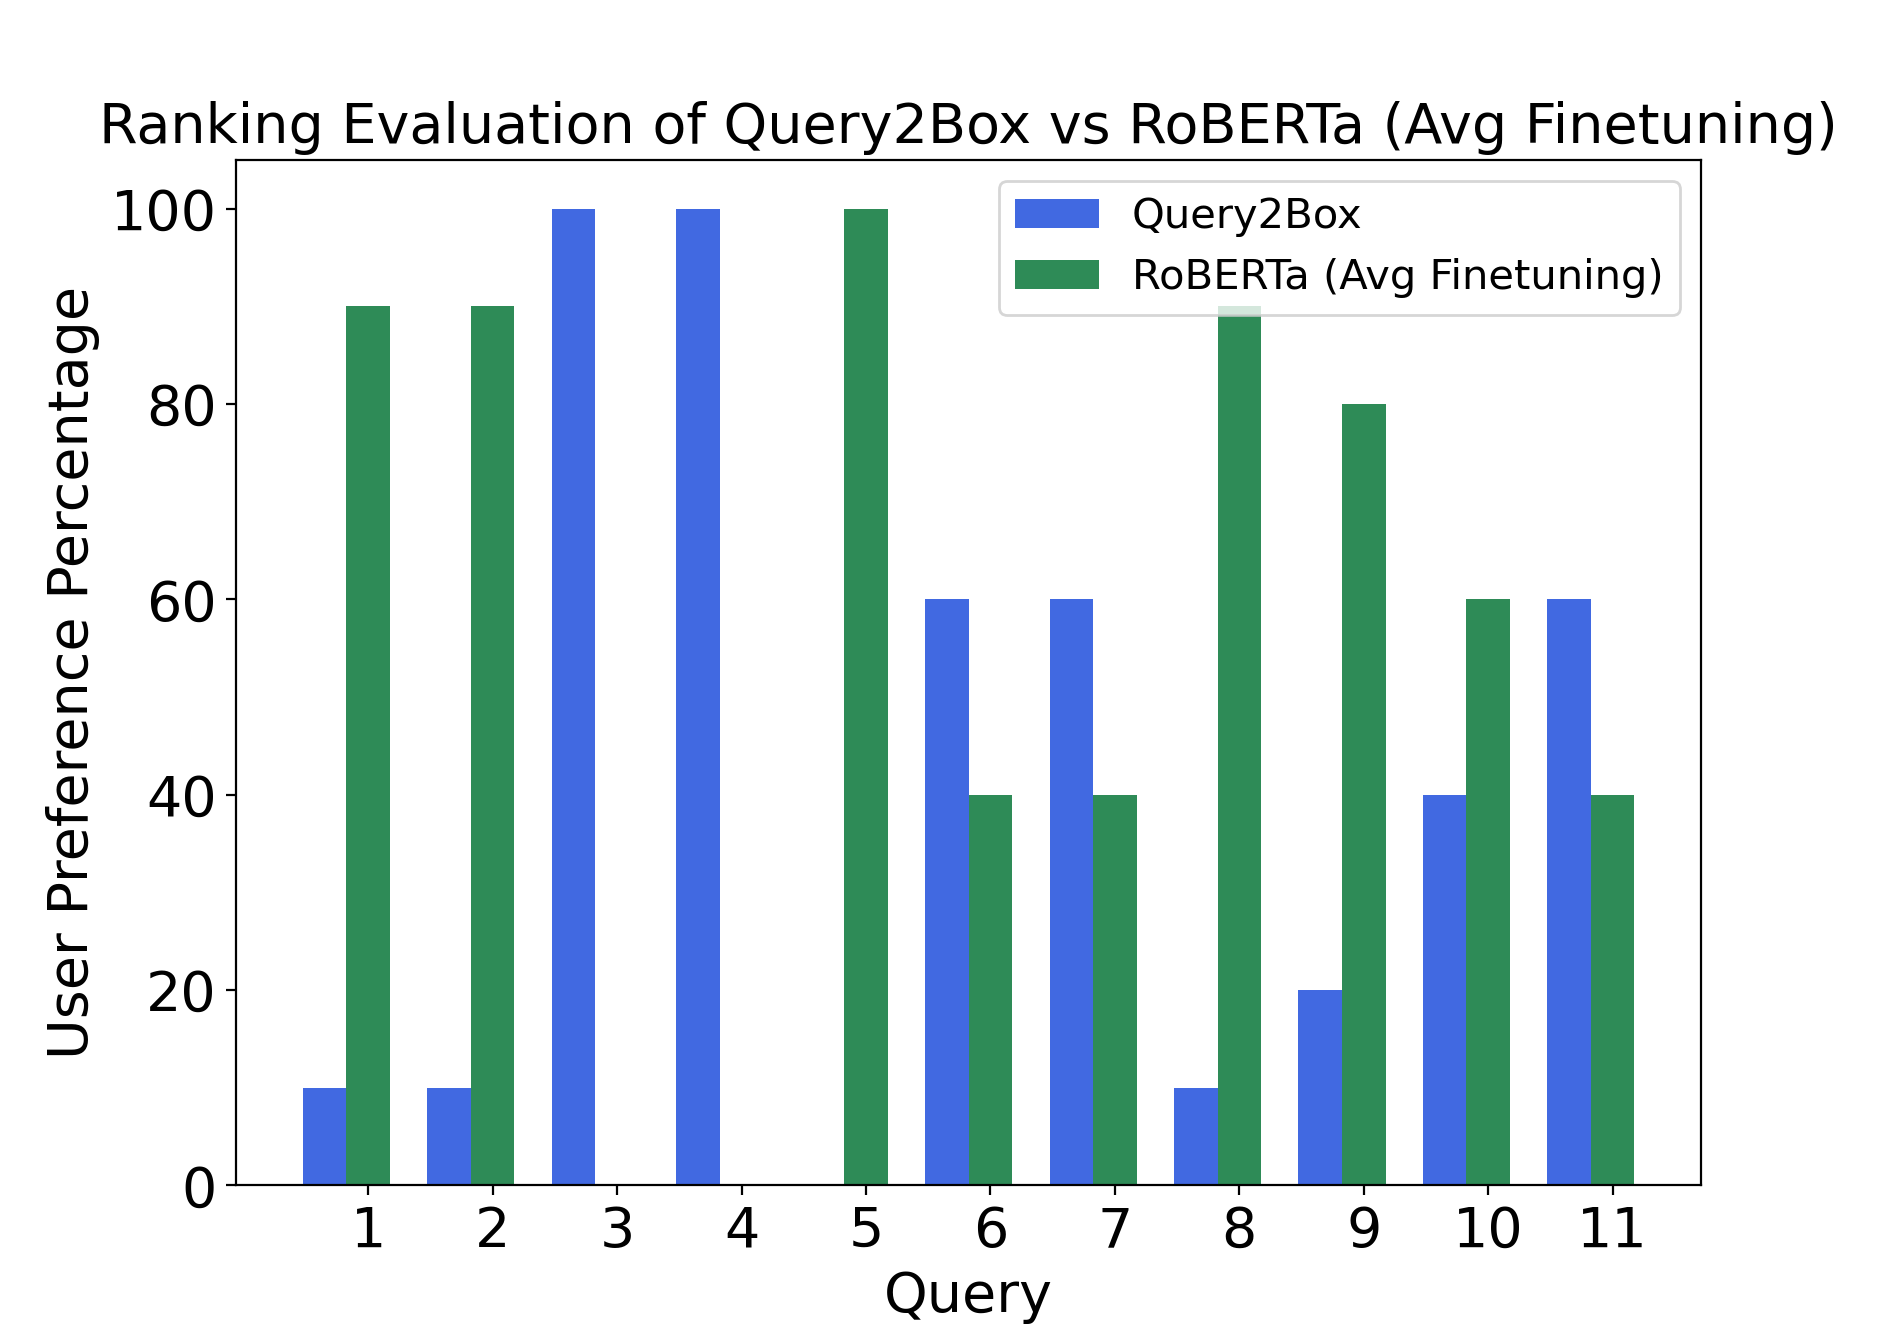
\includegraphics[clip,width=0.65\columnwidth]{submissions/Ali2023/figures/q2b_r2.png}%
% }
% ~
% \subfloat{%
%   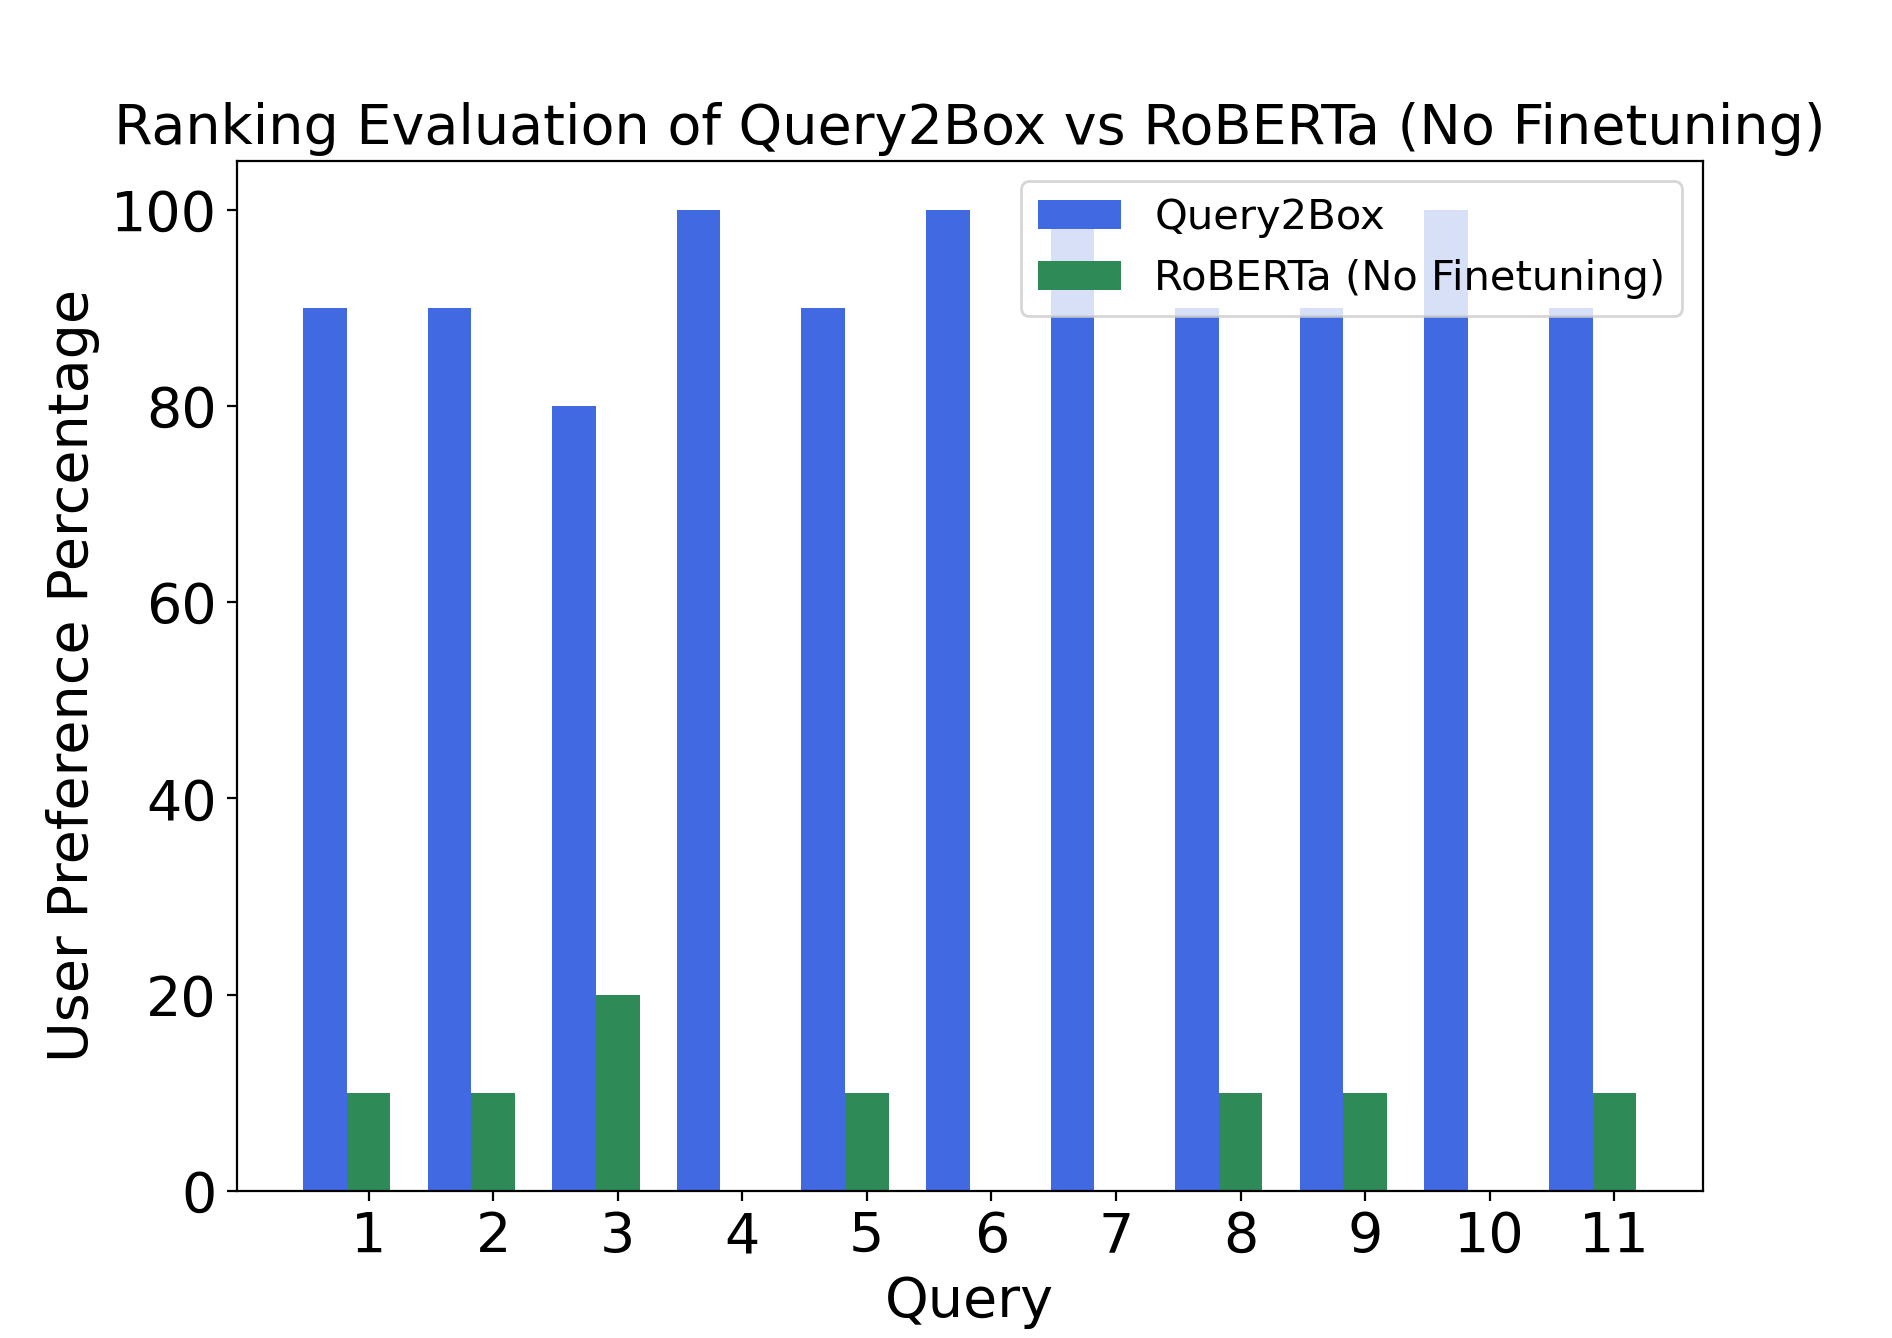
\includegraphics[clip,width=0.65\columnwidth]{submissions/Ali2023/figures/q2b_r3.png}%
% }
% \caption{Fact ranking using Query2Box vs. RoBERTa.}

% \label{fig:q2b_roberta}

% \end{figure*}

\begin{figure*}[!t]
\centering
\begin{minipage}{0.86\textwidth}
\begin{tabular}{@{}c@{}c@{}}
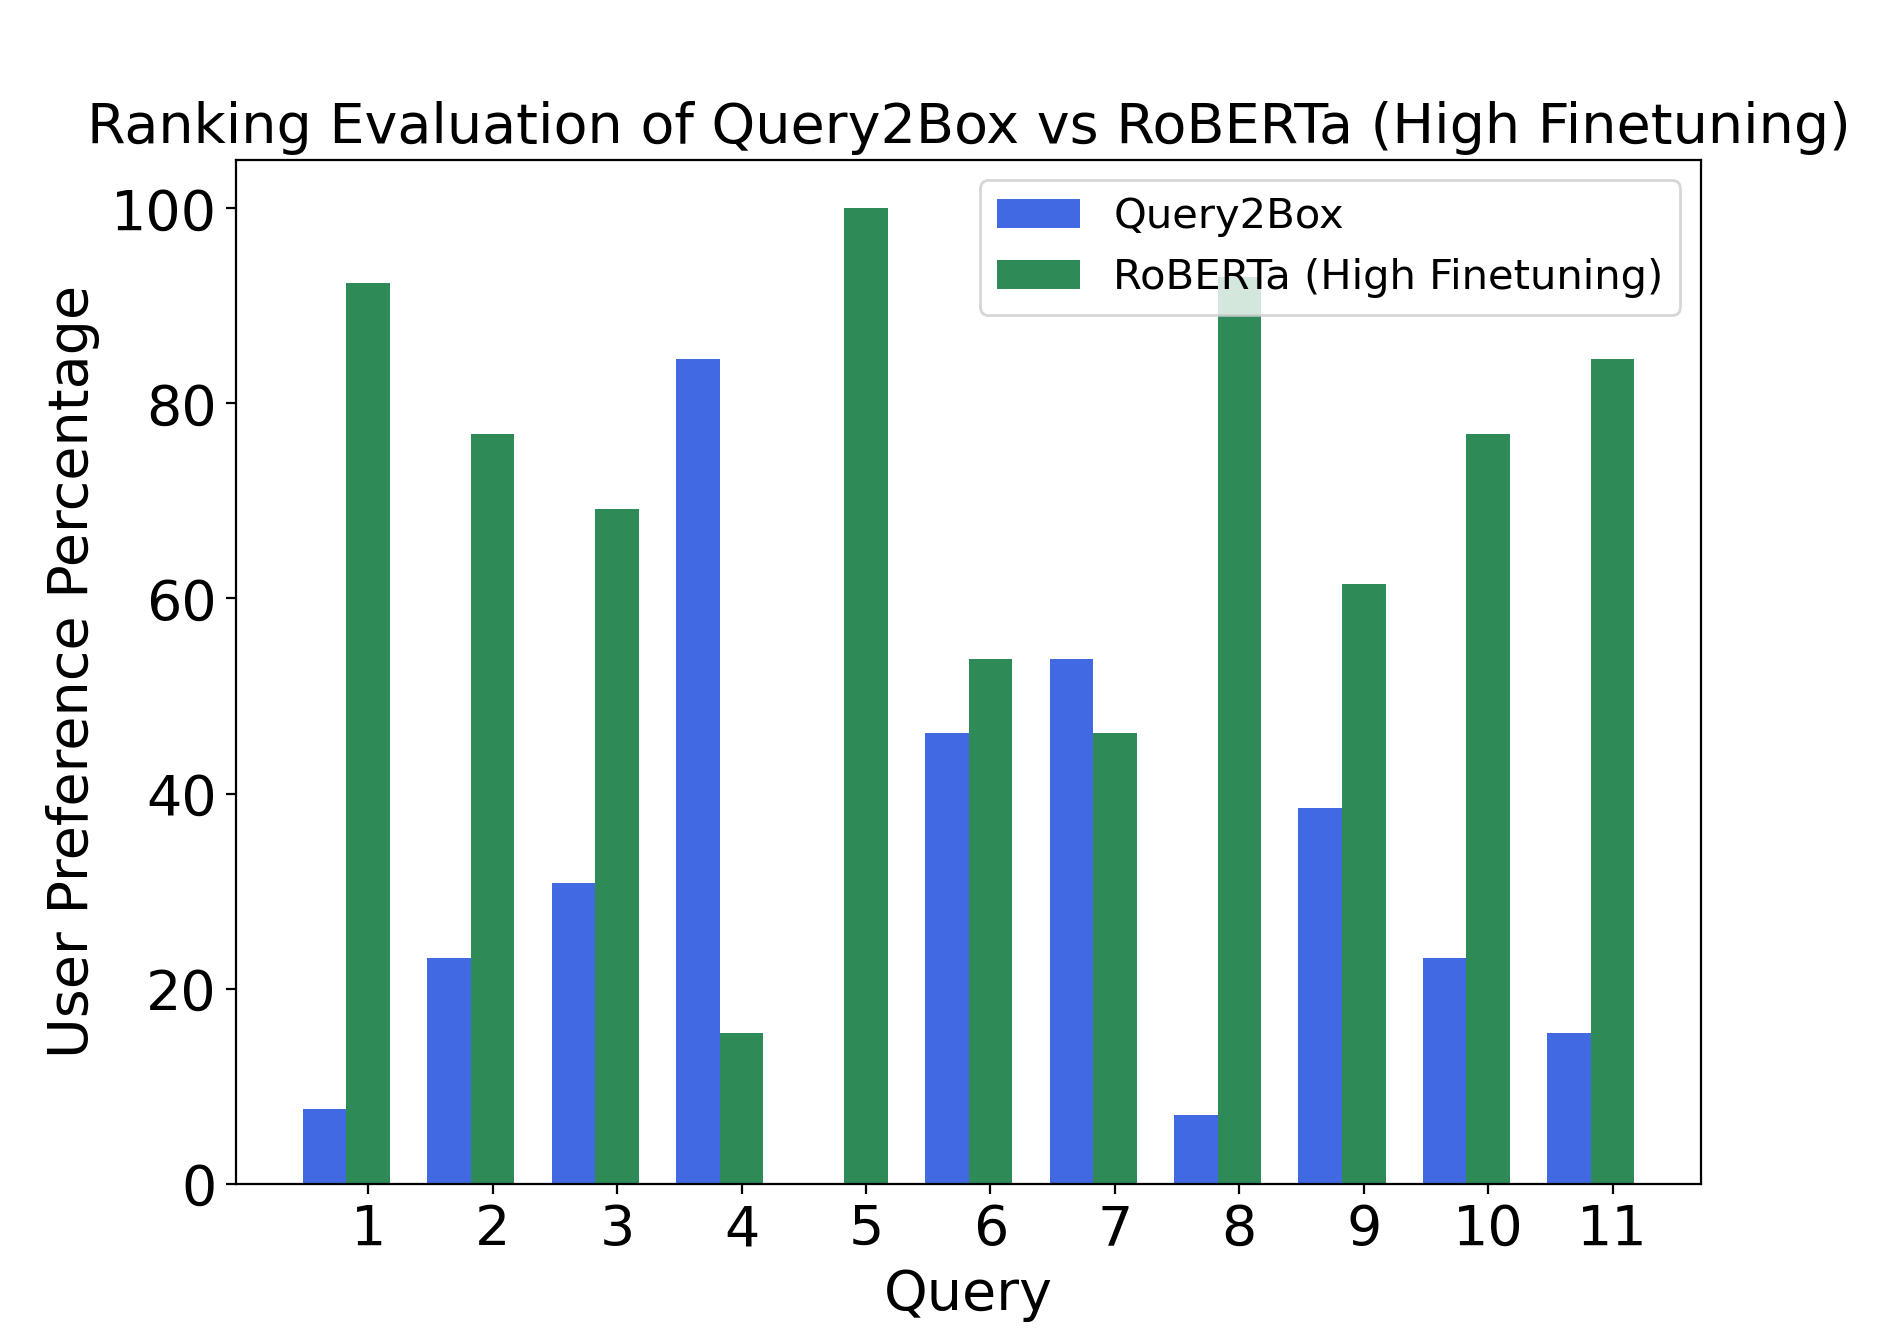
\includegraphics[width=0.43\textwidth]{submissions/Ali2023/figures/q2b_r1.png} & 
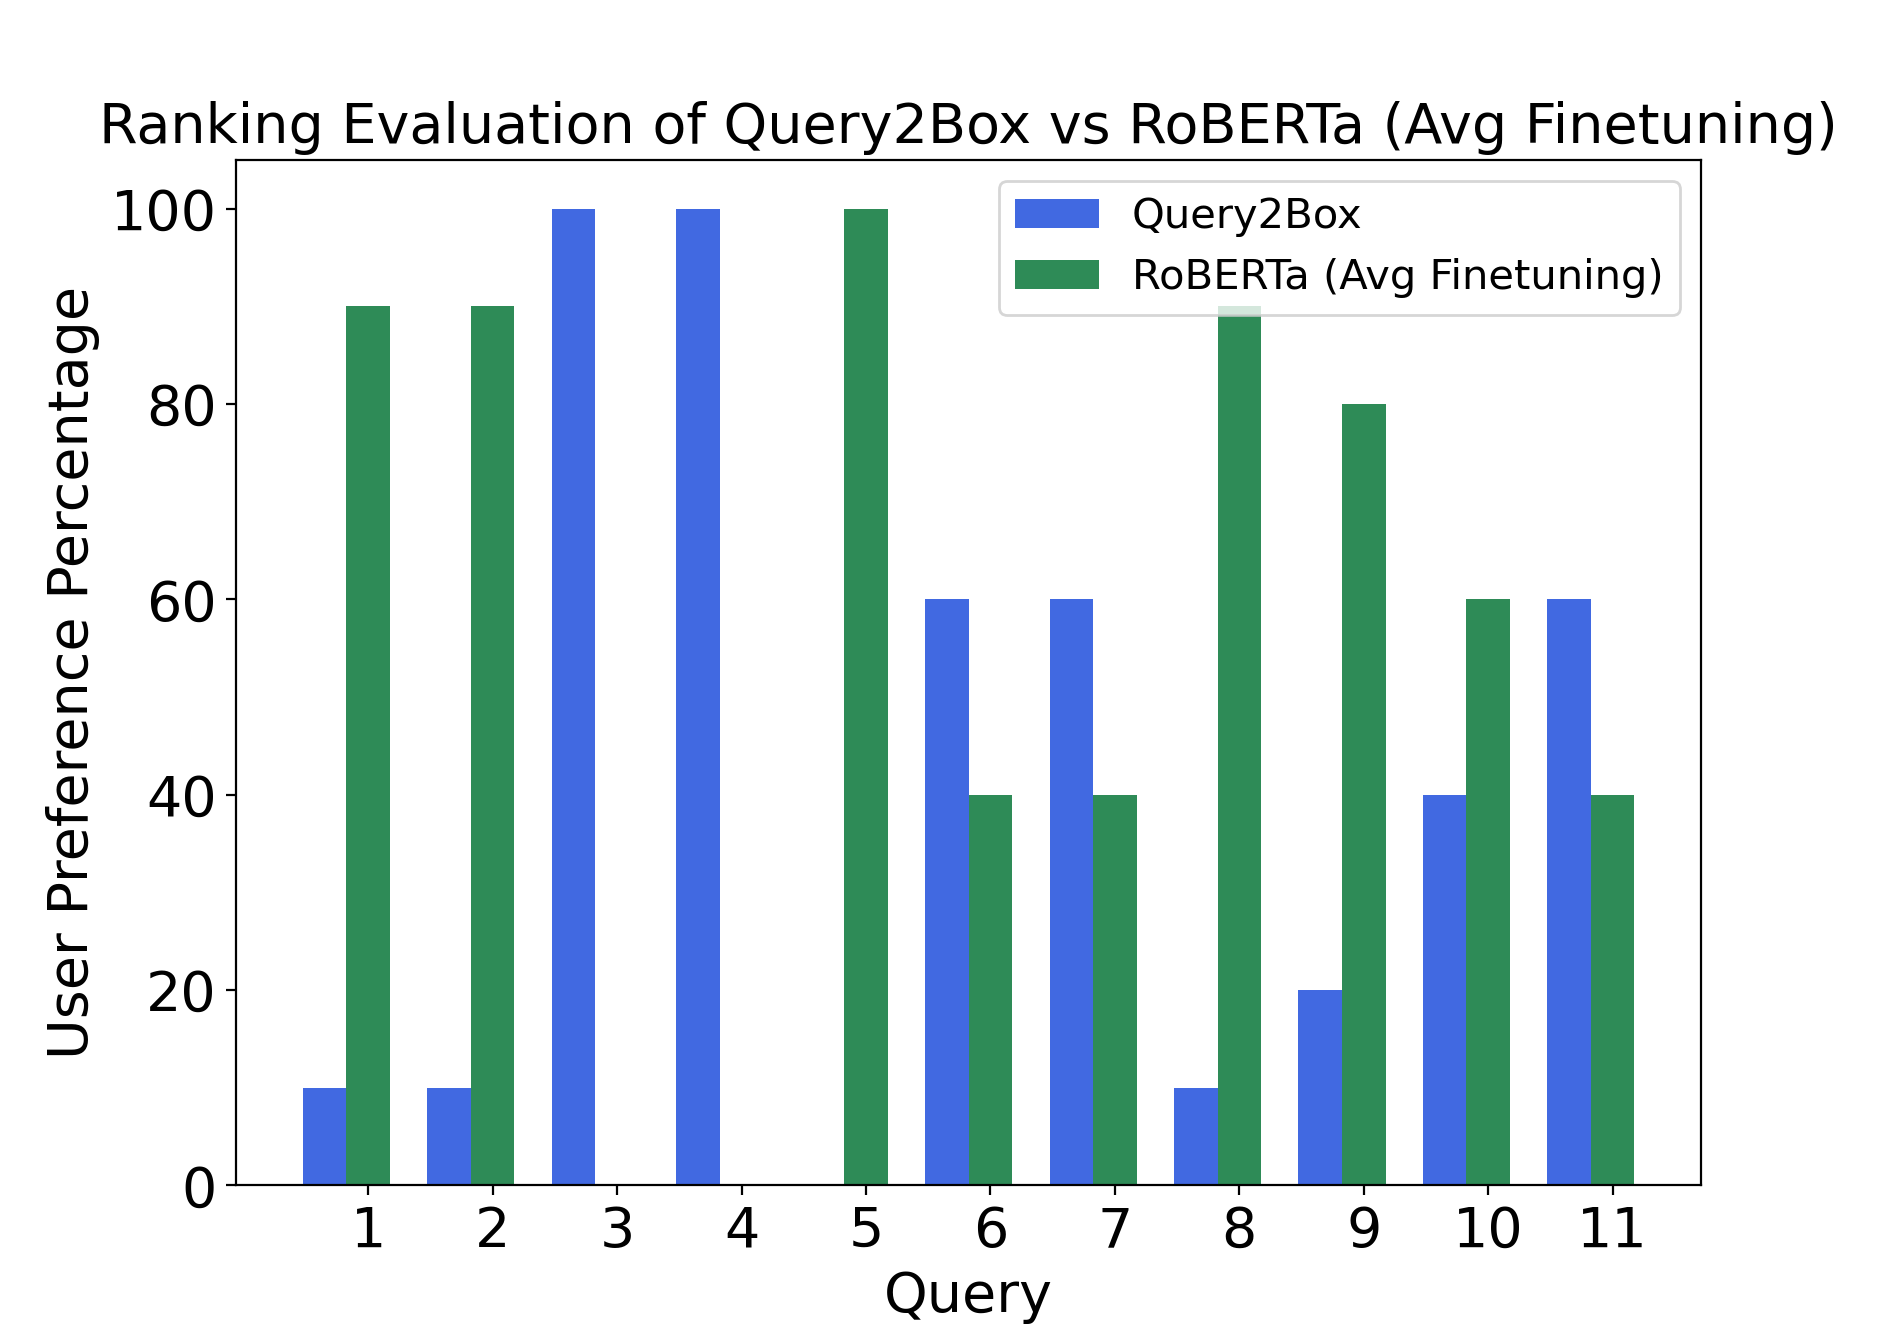
\includegraphics[width=0.43\textwidth]{submissions/Ali2023/figures/q2b_r2.png} \\
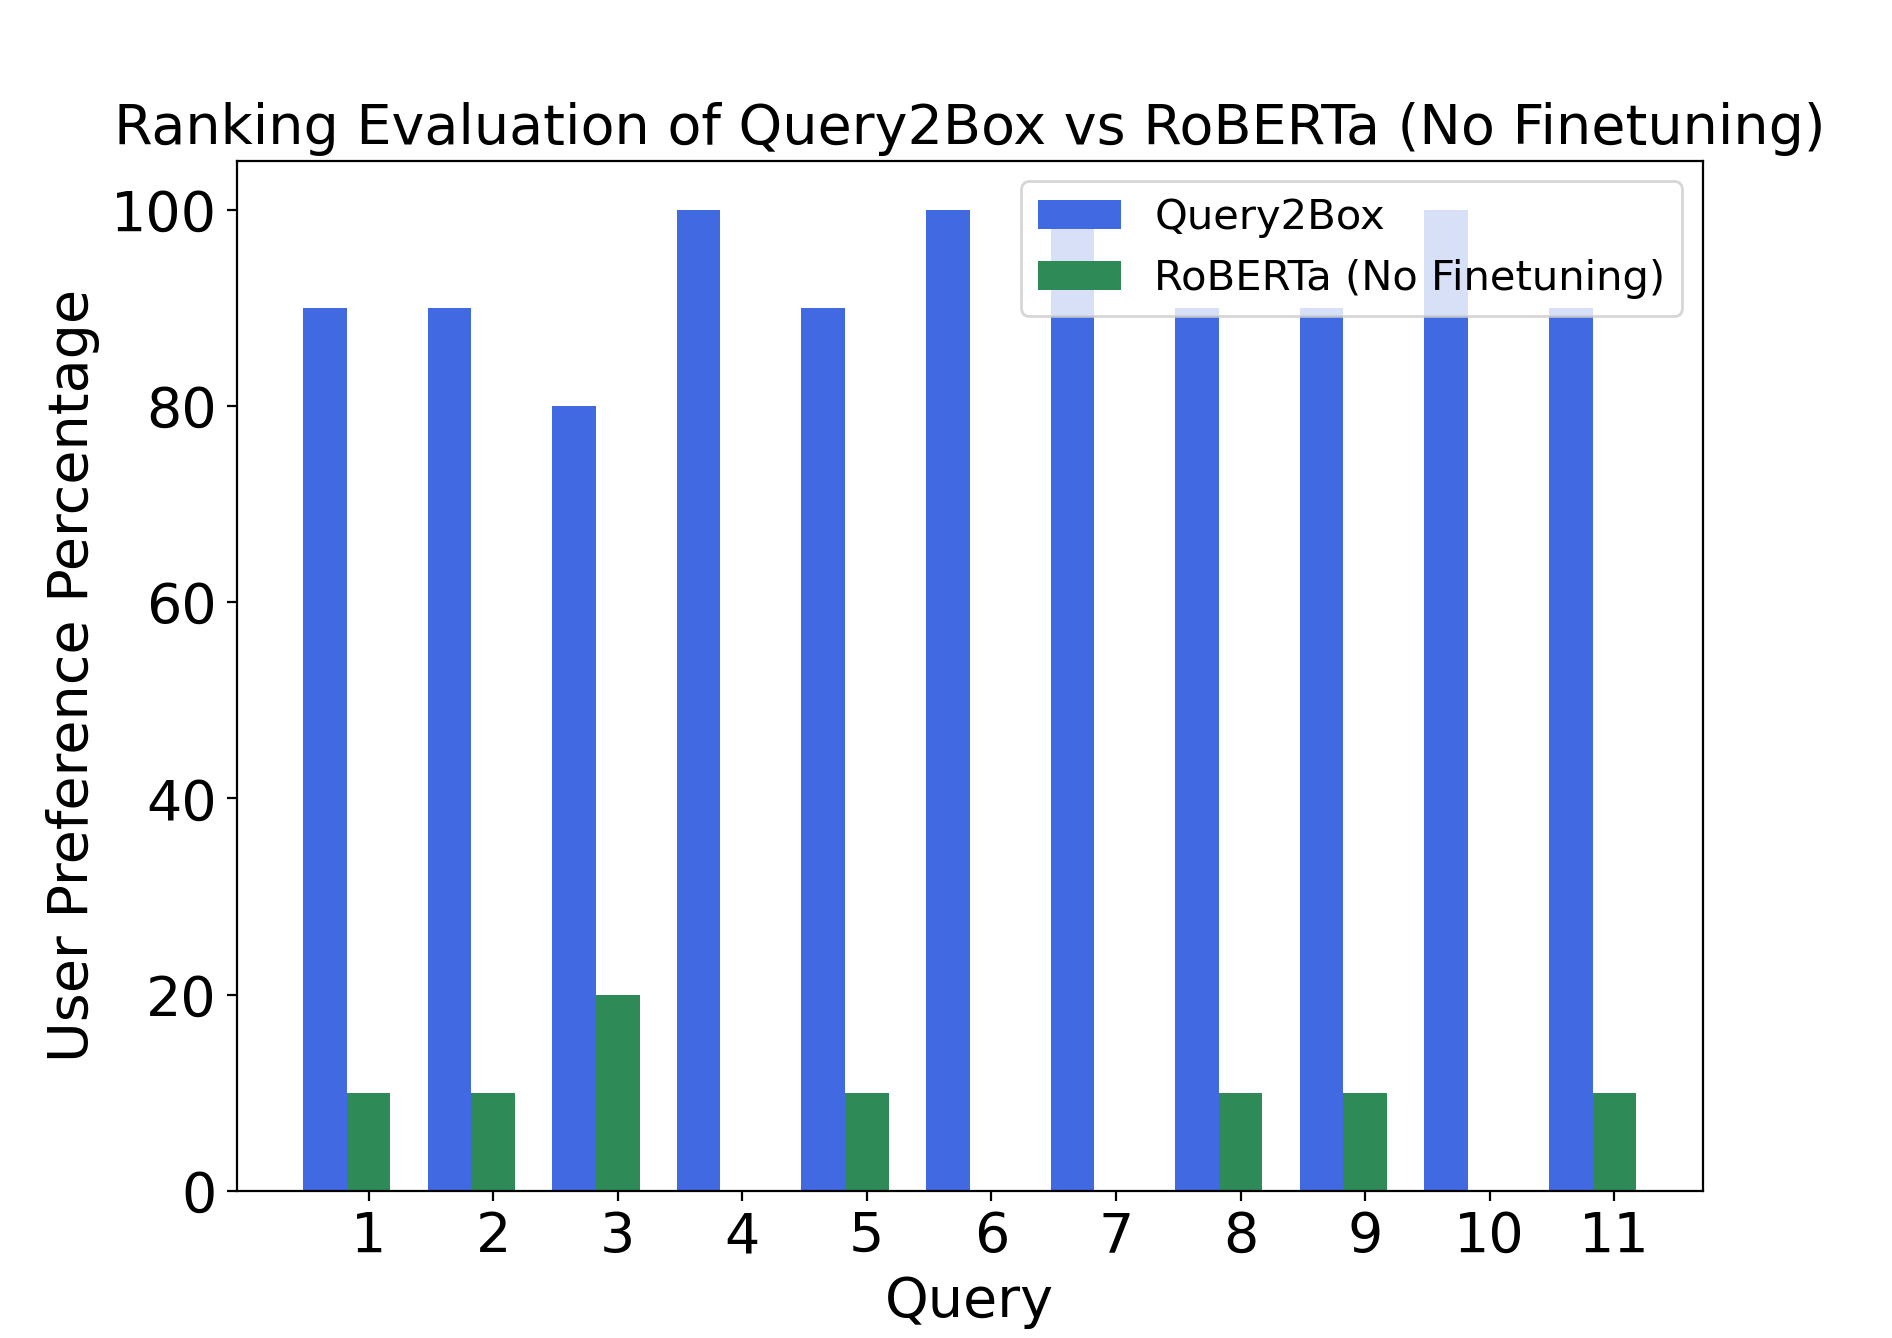
\includegraphics[width=0.43\textwidth]{submissions/Ali2023/figures/q2b_r3.png} &
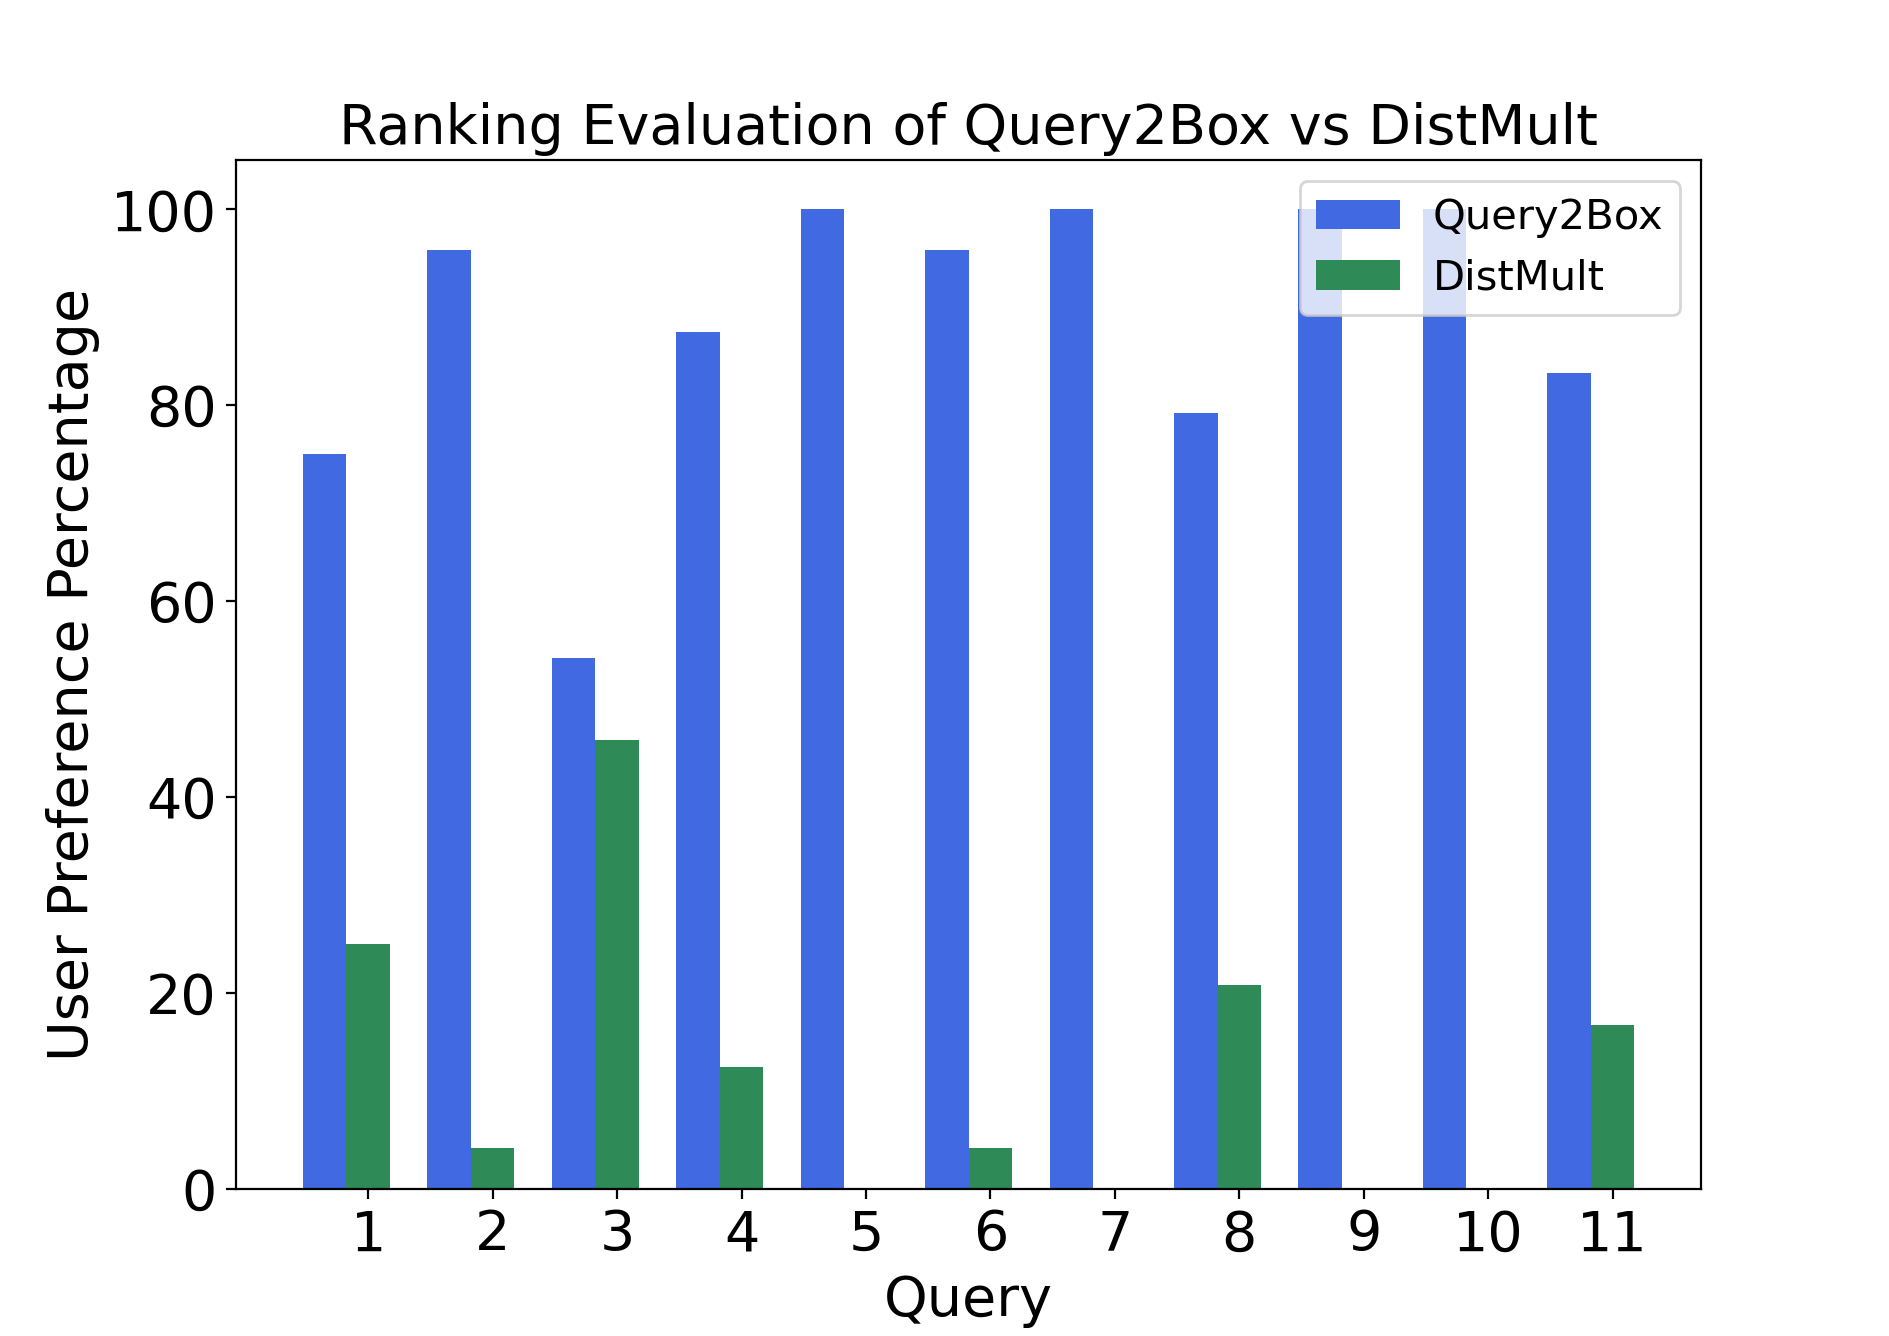
\includegraphics[width=0.43\textwidth]{submissions/Ali2023/figures/q2b_distmult.png}
\end{tabular}
\vspace{-3mm}
\caption{Fact ranking using Query2Box vs. RoBERTa and Query2Box vs. DistMult.
\label{fig:q2b_roberta_distmult}}
\end{minipage}
\end{figure*}







\begin{table}[t]
\caption{Average user preference (based on results in Figures \ref{fig:q2b_roberta_distmult}) for Q2Box vs other methods for different tasks. For RoBERTa models, (H): high finetuning, (A): average finetuning, (N): no finetuning.\label{tab:jen_ranking}}
\begin{tabular}{ccccc}
\textbf{Query2Box} & \textbf{DistMult} & \textbf{RoBERTa (N)} & \textbf{RoBERTa (A)}      & \textbf{RoBERTa (H)}      \\
\hline
1- TV Actor        & 1- Film Actor     & 1- Singer            & 1- Film Producer & 1- Actor         \\
2- Film Actor      & 2- Singer         & 2- Film Producer     & 2- Film Director & 2- Singer        \\
3- Film Director   & 3- Film Director  & 3- Film Director     & 3- Film Actor    & 3- Film Producer \\
4- Actor           & 4- Film Producer  & 4- Film Actor        & 4- TV Actor      & 4- Film Director \\
5- Film producer   & 5- Actor          & 5- Actor             & 5- Actor         & 5- Film Actor    \\
6- Singer          & 6- TV Actor       & 6- TV Actor          & 6- Singer        & 6- TV Actor     
\end{tabular}
\end{table}

\begin{table}[t]
\centering
\caption{Average user preference (based on results in Figure \ref{fig:q2b_roberta_distmult}) for Q2Box vs other methods for different tasks. For RoBERTa models, (H): high finetuning, (A): average finetuning, (N): no finetuning.}
\label{tab:avg_ranking}
\small
\begin{tabular}{@{}lccc@{}}
\textbf{Comparison Task} & \textbf{Competitor} & \textbf{Competitor Avg. Percentage} & \textbf{Q2Box Avg. Percentage} \\
\hline
DistMult / Q2Box         & DistMult            & 12\%                     & \textbf{88\%} \\
RoBERTa (H) / Q2Box      & RoBERTa (H)         & \textbf{70\%}            & 30\%          \\
RoBERTa (A) / Q2Box      & RoBERTa (A)         & \textbf{57\%}            & 43\%          \\
RoBERTa (N) / Q2Box      & RoBERTa (N)         & 7\%            & \textbf{93\%}          \\
\end{tabular}
\end{table}



% \begin{table*}[]
% \small
% \center
% \caption{Stability results of fact ranking. Query2box consistently achieves better performance than DistMult.}\label{tab:stability}
% \begin{tabular}{|l|c|c|c|c|ccc|}
% \hline
% \multicolumn{1}{|c|}{\multirow{2}{*}{}} & \multirow{2}{*}{Kendall} & \multirow{2}{*}{Weighted Kendall} & \multirow{2}{*}{Set-based Overlap} & \multirow{2}{*}{Rank-biased Overlap} & \multicolumn{3}{c|}{AdaptiveTau}                           \\ \cline{6-8} 
% \multicolumn{1}{|c|}{}                  &                          &                                   &                                    &                                      & \multicolumn{1}{c|}{0.02}  & \multicolumn{1}{c|}{0.05}  & 0.1   \\ \hline
% DistMult                                & 0.380                    & 0.384                             & 0.962                              & 0.990                                & \multicolumn{1}{c|}{0.460} & \multicolumn{1}{c|}{0.498} & 0.484 \\ \hline
% Query2box                               & \textbf{0.854}                    & \textbf{0.868}                             & \textbf{0.990}                              & \textbf{0.997}                                & \multicolumn{1}{c|}{\textbf{0.877}} & \multicolumn{1}{c|}{\textbf{0.917}} & \textbf{0.943} \\ \hline
% \end{tabular}
% \end{table*}



\begin{table}[!t]
\small
\center
\caption{Stability results of fact ranking. Query2box consistently achieves better performance than DistMult.}\label{tab:stability}
\begin{tabular}{cccccccc}
          & Kendall        & \begin{tabular}[c]{@{}c@{}}Weighted\\ Kendall\end{tabular} & \begin{tabular}[c]{@{}c@{}}Set-based\\ Overlap\end{tabular} & \begin{tabular}[c]{@{}c@{}}Rank-biased\\ Overlap\end{tabular} & \begin{tabular}[c]{@{}c@{}}AdaptiveTau\\ $\delta'=0.02$\end{tabular} & \begin{tabular}[c]{@{}c@{}}AdaptiveTau\\ $\delta'=0.05$\end{tabular} & \begin{tabular}[c]{@{}c@{}}AdaptiveTau\\ $\delta'=0.1$\end{tabular} \\ \hline
DistMult  & 0.380          & 0.384                                                      & 0.962                                                       & 0.990                                                         & 0.460                                                                & 0.498                                                                & 0.484                                                               \\
Query2Box & \textbf{0.854} & \textbf{0.868}                                             & \textbf{0.990}                                              & \textbf{0.997}                                                & \textbf{0.877}                                                       & \textbf{0.917}                                                       & \textbf{0.943}                                                     
\end{tabular}
\end{table}


\section{Experiments}\label{sec:ali_experiment}
We evaluate reasoning-based KG embeddings for fact ranking. We focus on fact ranking tasks that align with use cases in industrial deployments. We evaluate the following aspects of our proposed framework: (1) the utility to end users when using KG embeddings for fact ranking, (2) the stability of KG embedding models and hence to what extent they satisfy deployment requirements.

\subsection{Experiment Setup}

\newparagraph{Queries and Facts}
We focus on queries of the format \qu{What is the occupation of \texttt{[Celeb\_Name]}?} which captures the ranking task. We rank possible object completions for the structured query $(v_s, \texttt{OccupationOf}, ?)$, where $v_s$ is the entity of interest. Our dataset contains several million queries obtained by real intelligent assistant user queries.

\newparagraph{Knowledge Graph}
We consider the entire Wikidata KG~\cite{wikidata} to validate the proposed framework. The version of Wikidata that we use contains 1,754,058,566 facts defined over 91,900,599 entities and 35,446 relation types. We train our framework on this KG and obtain the answers to the aforementioned set of user queries by finding entities in this KG.

\newparagraph{Baselines}
We evaluate a diverse array of methods, including KG reasoning embeddings \textit{Query2box}~\cite{ren2020query2box}, shallow KG embeddings \textit{DistMult}~\cite{distmult},  and masked language models (MLMs) \textit{RoBERTa}~\cite{liu2019roberta}. 

For KG embedding based methods, both DistMult and Query2box fit in our unified framework. We adopt the standard training procedures for these models (see Section~\ref{sec:ali_prelim}). \iffalse Specifically, we randomly initialize the entity embedding matrix $\rmV_\theta$ and the relation embedding matrix $\rmR_\theta$ for both models. \fi For DistMult, we sample existing edges as positive samples and non-existing edges as negative samples to train the DistMult model with the objective defined in \eqref{eq:kgelossfunc}, where the distance and residue functions are defined in \Secref{sec:ali_prelim}. For Query2box, similar to~\cite{ren2020query2box} and as discussed in \Secref{sec:ali_background}, we sample multi-hop queries (\Figref{fig:query}), and their answers and non-answers to optimize the contrastive objective in \eqref{eq:lossfunc}. Besides the entity and relation embedding matrices, we use the neural logic operators in Query2box to embed the complex queries and optimize the query embeddings such that they are close to the answer embedding and pushed far away from the embedding of the sampled non-answers. We use the distance function of the original Query2box model and design the residue function as described in \Secref{sec:ali_prelim}.








For both DistMult and Query2Box, we use SMORE~\cite{ren2021smore} for training. We train both for 100k iterations with the Adam optimizer~\cite{kingma2014adam}. We anneal the learning rate from 0.001 to 0.0001, and adopt a batch size of 8,192 queries with 1,024 negative answers for each query in the batch.
\iffalse Given queries about a celebrity's occupation, \ie, $(v_s, \texttt{OccupationOf}, ?)$ and a candidate answer $v_o$,\fi
We score each candidate answer using the distance functions defined for both models.

For MLMs, we use the RoBERTa model. Given a triple-format query $(v_s, \texttt{OccupationOf}, ?)$, we provide three templates and convert the query into a natural language question. These templates include (1) \qu{$v_o$ is a {\tt [mask]}.}, (2) \qu{The occupation of $v_o$ is {\tt [mask]}.}, and (3) prompting~\cite{wei2021why} in which the template is \qu{Barack Obama is a politician, LeBron James is a basketball player, $v_o$ is a {\tt [mask]}.}. For different query types, we need to provide different prompts in order to make predictions more effective. As we show later, fine-tuning of the prompt is necessary to obtain competitive results and hence, MLMs are not a universal solution to our task. Given $v_o$, we score the candidate answer by calculating the likelihood score of $v_o$ in replacement of the \texttt{[mask]} in each of the three templates.


\subsection{Fact Ranking Evaluation}\iffalse We evaluate the utility and stability of our framework.\fi

\newparagraph{Utility}
We first evaluate the utility of our framework on the fact ranking task. \iffalse In fact ranking, we aim to use our framework to output a ranked list of answers to the input queries. As we mentioned in \Secref{sec:ali_ranking}, the first requirement for this task is to have a model whose outputs align well with user expectation. Therefore, in order\fi To assess the quality of Query2Box and compare it against other methods, we consider eleven celebrities and their occupations as listed in WikiData. We present our users with four different questionnaires. Each of these questionnaires compares Query2box ranking vs. another baseline ranking obtained using one of the methods we mentioned earlier. Each questionnaire contains eleven questions where each asks users to choose between two different rankings (Query2Box vs. a baseline) of a celebrity occupation.


\Figref{fig:q2b_roberta_distmult} shows the summary of user preferences between DistMult/RoBERTa and Query2box rankings. In \Figref{fig:q2b_roberta_distmult}, Query2box has outperformed DistMult and Query No. 3 (occupations of Jennifer Lawrence) shows the tightest competition. Table \ref{tab:jen_ranking} shows the ranking derived from these methods. Jennifer Lawrence is mostly known as a \textit{Film Actor} which is correctly predicted by DistMult. Some users have focused on the first occupation and hence voted for DistMult while other users have considered other occupations and voted for Query2box. In addition, we can notice the flipping of user preferences based on the amount of fine-tuning for RoBERTa models (see also Table \ref{tab:avg_ranking}). As shown in Table \ref{tab:avg_ranking} which represents the average user preference, Query2Box outperforms DistMult and RoBERTa requires significant fine-tuning of the prompt to outperform the Query2box model.


\begin{comment}

\textcolor{red}{fact verification figure commented out}
\begin{figure*}
        \centering
      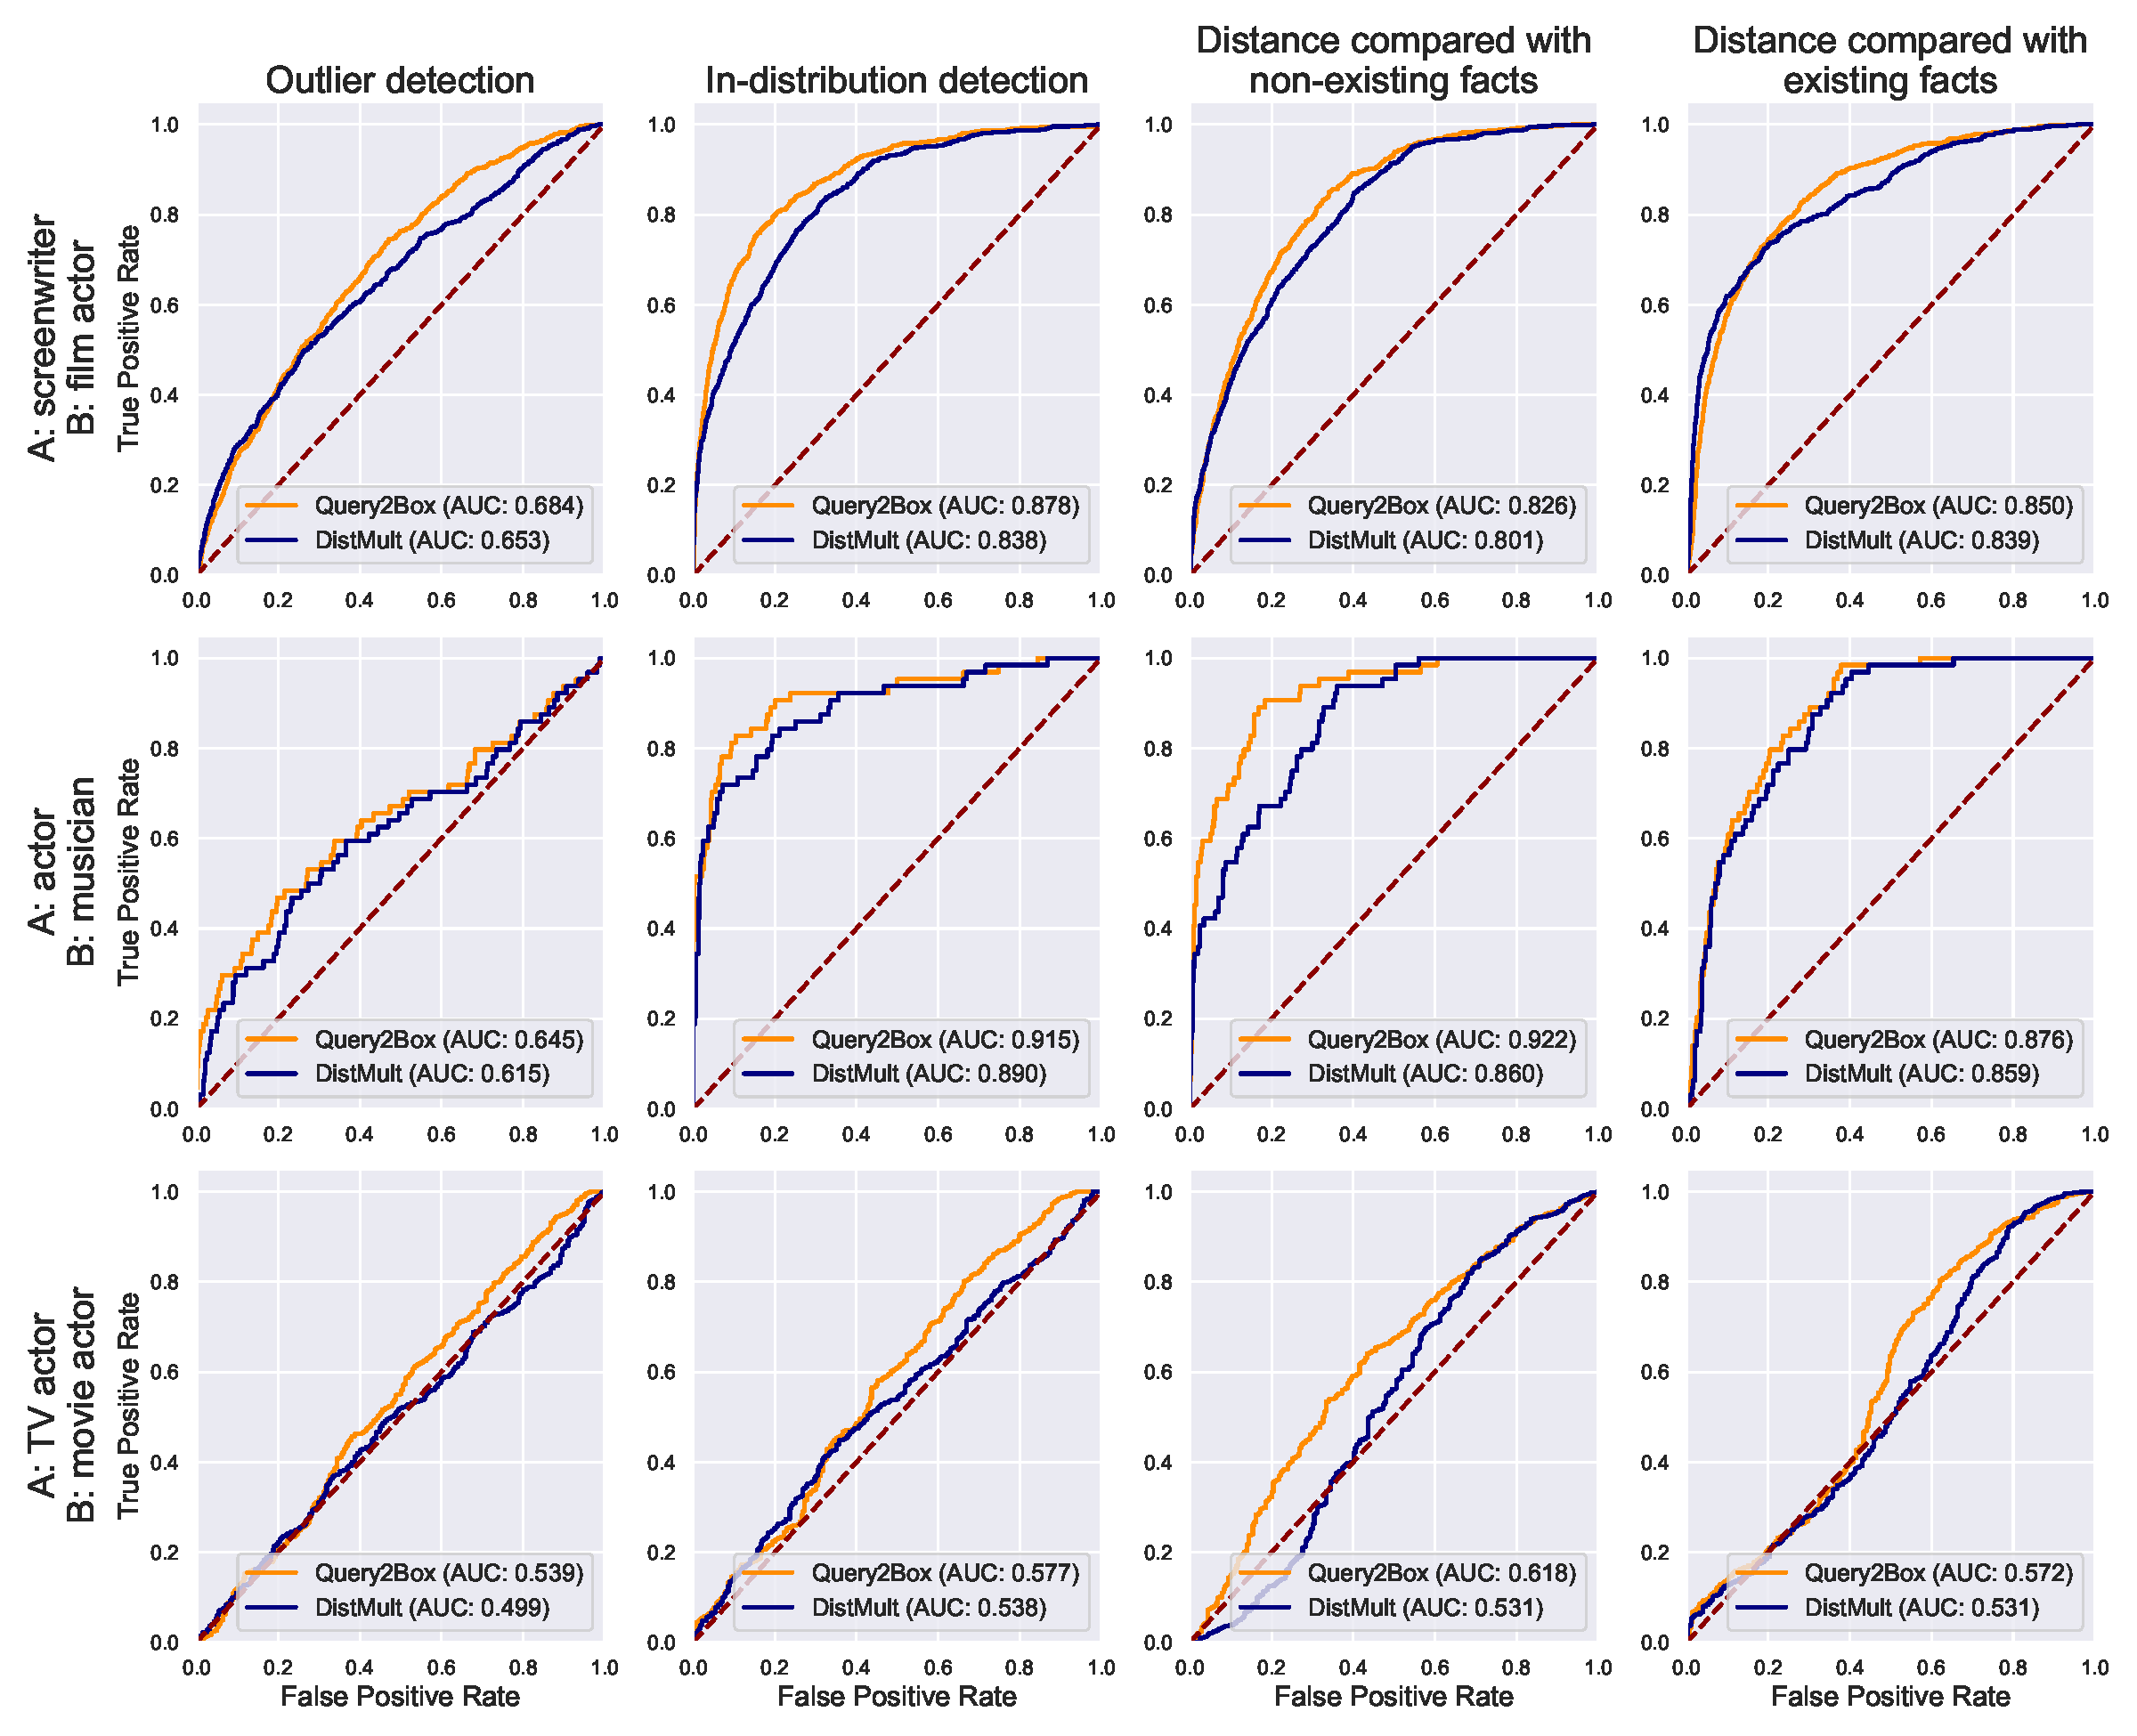
\includegraphics[width=1.7\columnwidth]{submissions/Ali2023/figures/final_roc.pdf}
      \caption{ROC-AUC curve of Query2box and DistMult in three case studies in fact verification. Query2box consistently achieves better performance than DistMult across cases and metrics. }
    \label{fig:roc-verification}
\end{figure*}
\end{comment}



\newparagraph{Stability}
We now measure the stability of different systems using the metrics we introduced in \Secref{sec:ali_method}.
We take all triples with \texttt{OccupationOf} as the relation type from the massive KG. Overall the dataset involves 6,566,224 queries of structure $(v_o, \texttt{OccupationOf}, ?)$ for which we measure the stability and consistency of rankings\iffalse across multiple runs (of training) for each method of interest\fi. 
Here we mainly consider two methods Query2box and DistMult, but not the MLMs due to their necessity of contexts for better ranking utility as discussed.
We train both models 5 times and measure the stability of both models using the metrics introduced in \Secref{sec:ali_consistency}.
As shown in Table \ref{tab:stability}, we find Query2box is more stable and consistent than DistMult since Query2box is trained on more complex multi-hop queries, which better captures the neighborhood structure for each fact.
\iffalse Specifically, for all the Kendall's Tau based methods (original, weighted or adaptive), Query2box is 0.474, 0.484, 0.432 better than DistMult.\fi For set-based overlap and rank-biased overlap, both methods achieve extremely high values. This is expected since the occupations of a celebrity are fixed across runs, and the overlap will always be 1 at the last step as we gradually compare the intersection of two sets starting from top-ranking items to the low-ranking ones.
Among evaluation metrics, our adaptive method can better characterize a more meaningful measurement of ranking stability than the vanilla Kendall's Tau and rank-biased overlap. As shown in Table \ref{tab:stability}, Query2box achieves higher performance in AdaptiveTau than the other two metrics. We argue such an adaptive metric is crucial in evaluating ranking stability in production. %Finally, we defer the experimental results for fact verification to \Secref{sec:ali_fact_ver_eval}.

\iffalse
\subsection{Performance  Improvements for Related Entity Search}
\revise{
We now present the performance improvements our hybrid query processing optimizations described in Section \ref{sec:ali_system}. We use a subset of KG entity embedding vectors, and compare the performance of our system against available existing hybrid query processing strategies (see \cite{mohoney2023high} for more details) using a randomly sampled and aggregated query workload from anonymized, historical queries. As shown in Table \ref{tab:end_to_end}, \hybridindex provides orders of magnitude performance improvements over best performing baselines for the related entity search task.
}

\begin{table}[t]
\small
\centering
	\caption{Slowdown for related entity search compared to \hybridindex @ Recall $>= .8$}\label{tab:end_to_end}
	\begin{tabular}{| c | c | c | c | c |}
		\hline
		 & \hybridindex & PreFilter & PostFilter & Range \\
		\hline
		\hline
		Slowdown & $1\times$ & $31\times$ & $136\times$ & NA \\
        \hline
	\end{tabular}
\end{table}
\fi
%%%%%%%%%%%%%%%%%%%%%%%%%%%%%%%%%%%%%%%%%%%%%%%%%%%%%%%%%%%%%%%%%%%%%%%%%%%%%%%%%%%%%%%%%%%%%%%%%%%%%%%%%%%%%%
\iffalse


\begin{figure*}
        \centering
      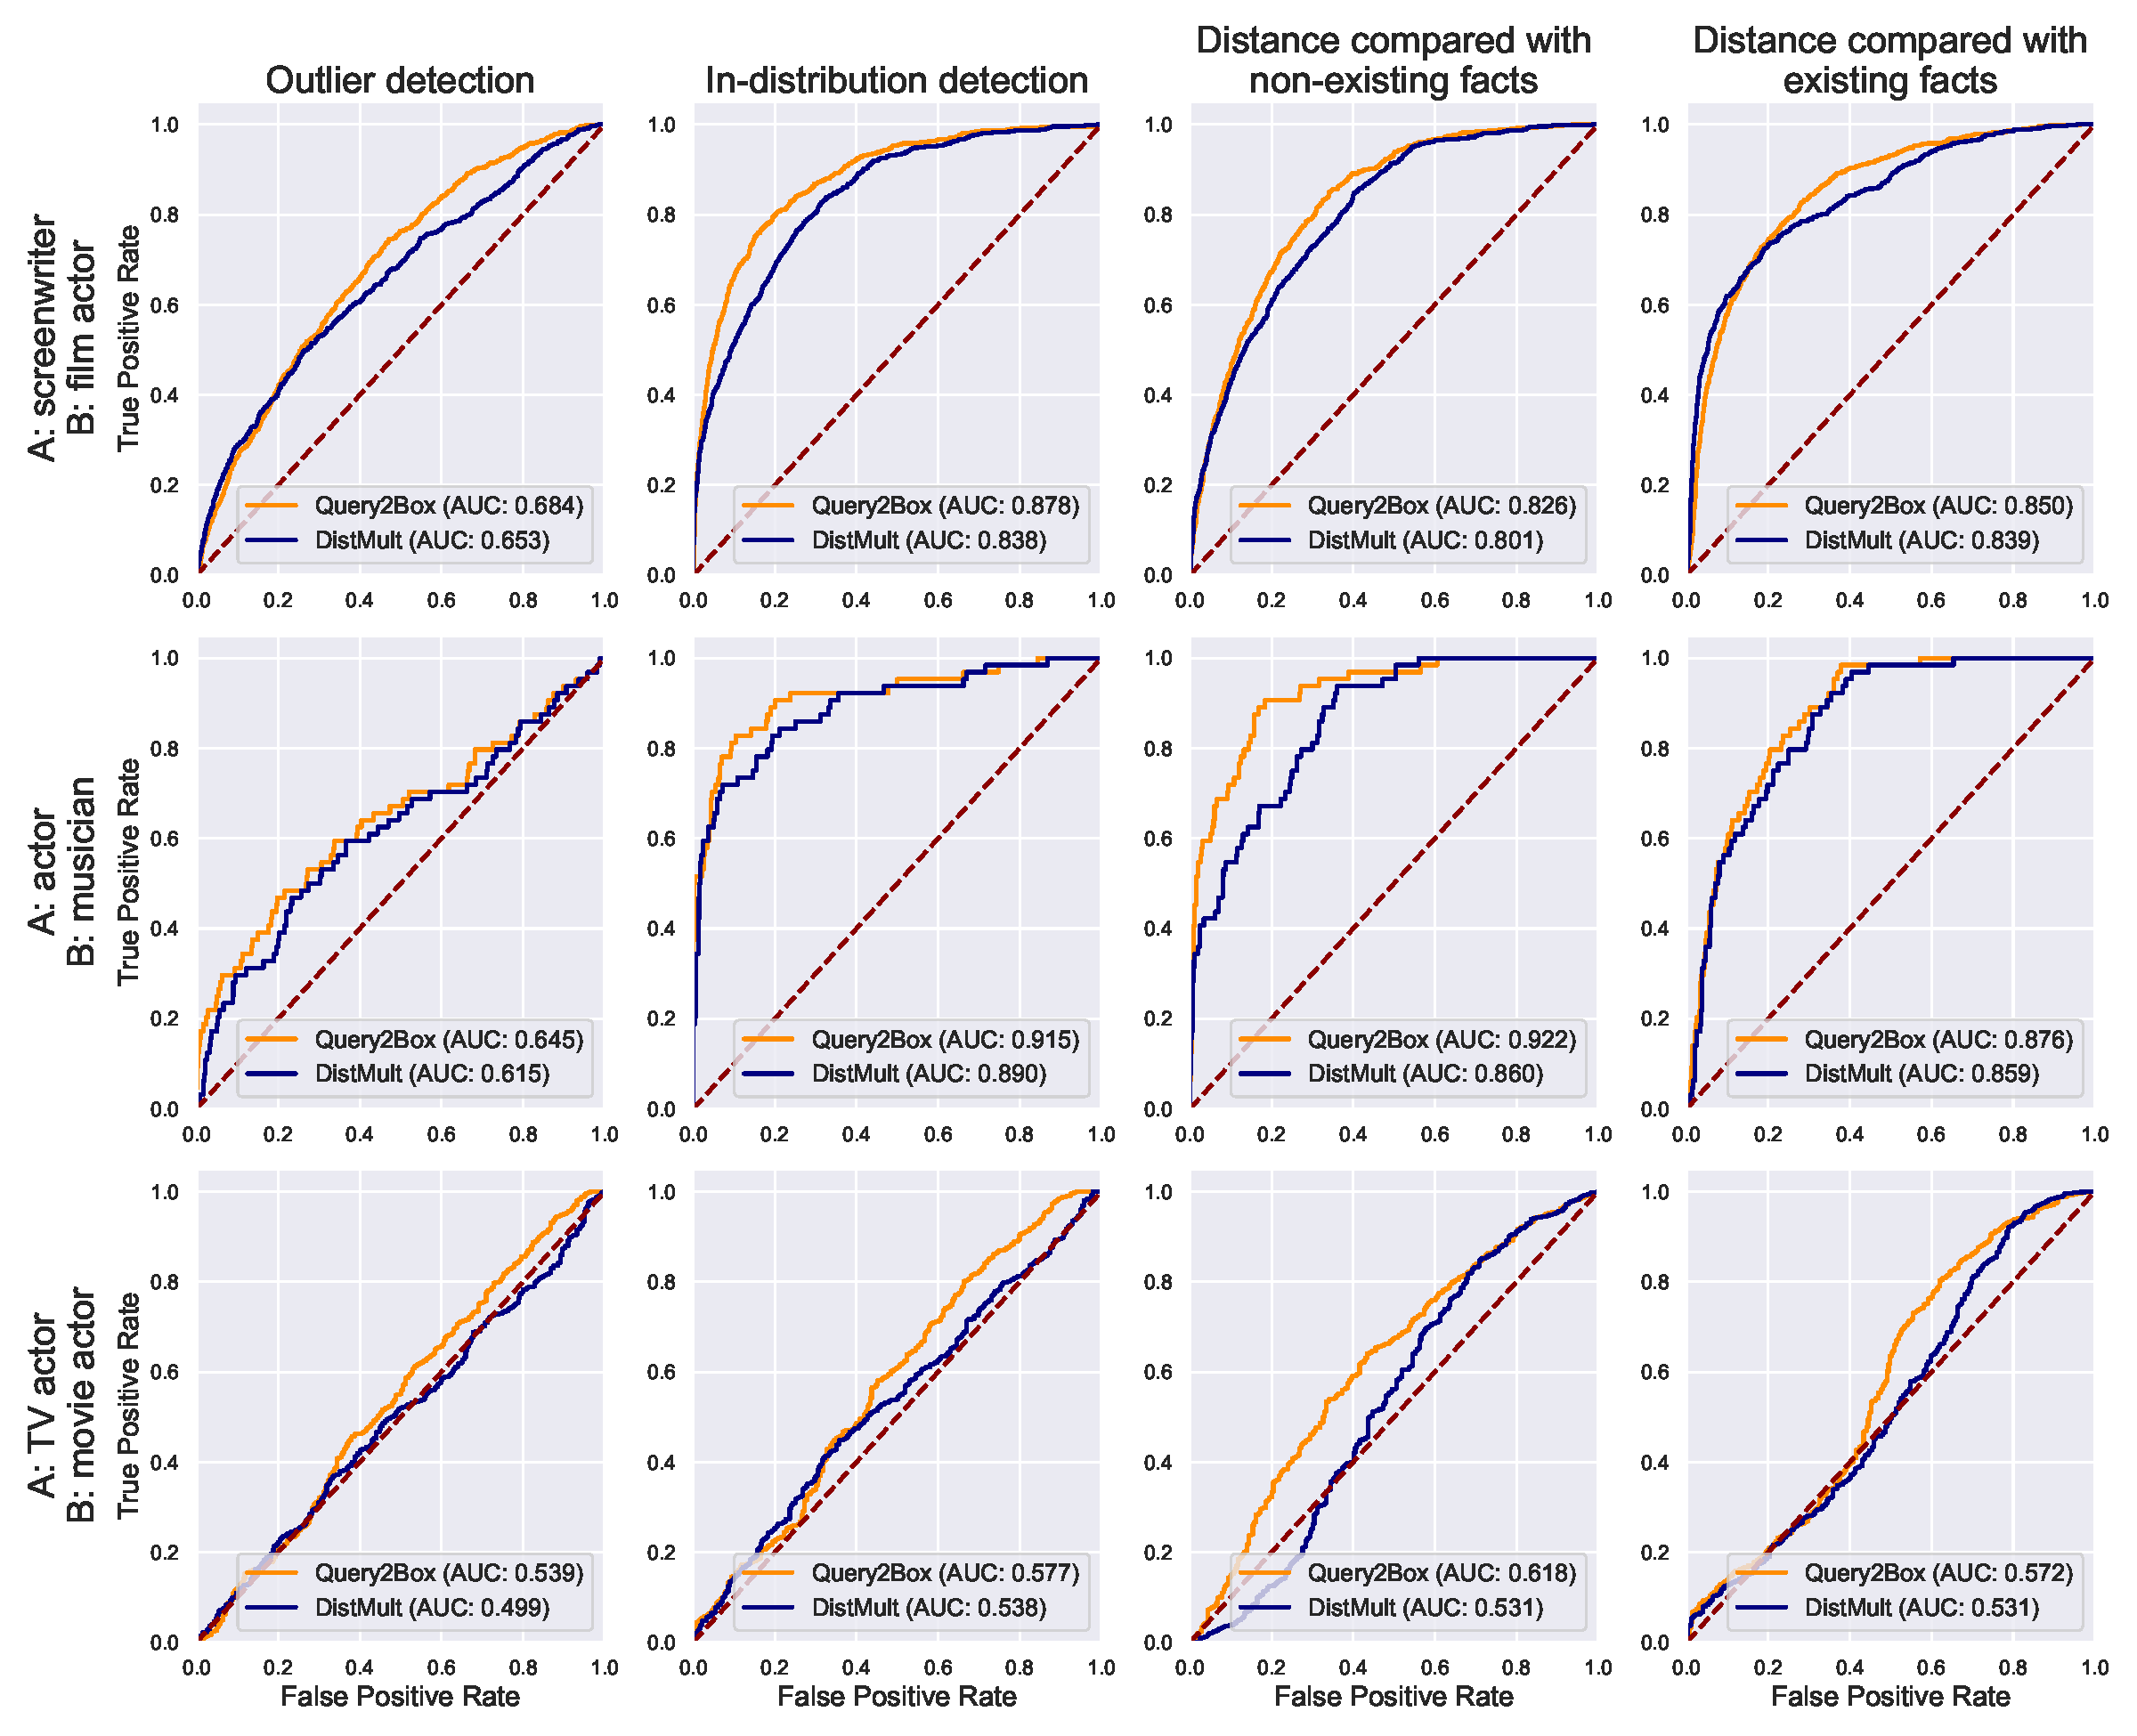
\includegraphics[width=1.5\columnwidth]{submissions/Ali2023/figures/final_roc.pdf}
      \caption{ROC-AUC curve of Query2box and DistMult in three case studies in fact verification. Query2box consistently achieves better performance than DistMult across cases and metrics. }
    \label{fig:roc-verification}
\end{figure*}


\section{Fact Verification Evaluation}\label{sec:ali_fact_ver_eval}
% Here we conduct experiments on the fact verification task. 
% Verifying the existing and missing facts on KG is one of the most important tasks in real-world production. Instead of giving a set of triplet facts directly for human curators to verify, we propose using our framework so that we can prioritize the promising facts for human curators to check first. 
We focus on queries about the occupation of a given celebrity with three case studies in fact verification task. In each case study, our system is given a set of celebrities $\{v_s\}$ of an occupation $A$, and the goal is to identify which celebrities among the set are likely to have occupation $B$. 
As introduced in \Secref{sec:ali_calibration}, we execute three different methods to calibrate the scores in our system. These methods include (1) outlier detection 
% -- we estimate a Gaussian distribution over sampled non-existing facts and verify whether a fact is an outlier to them using the Mahalanobis distance; 
(2) in-distribution sample detection 
% -- we sample existing facts related to the fact to verify and check whether the fact is an in-distribution sample; 
(3) distance compared with related facts.
% -- we calculate the score of a triplet fact (\ie, distance between the query and object as in \eqref{eq:lossfunc}, and also obtain the score of the sampled related facts, and compare to what extent the score of the fact is higher than that of the related facts. 
% For the method (3), we also use two definitions of related facts, including non-existing facts (same celebrity $v_s$ and relation {\tt OccupationOf} with an object entity $v_o$ where $(v_s, \texttt{OccupationOf}, v_o)$ does not exist on the graph) or existing facts (a set of $(v_s, \texttt{OccupationOf}, v_o)$ where $v_s$ is a semantically similar celebrity and the fact exists on the graph).


\newparagraph{Case study I -- A: screenwriter, B: film actor}
The first case study is that we aim to predict which celebrities in the given set of screenwriters are more likely to be also film actors. This case study is extremely challenging since screenwriters and film actors do not have a strong correlation, \ie, knowing a person is screenwriter does not give much information about whether this person is also a film actor. Together we have 5,715 screenwriters and we ask the human curators to first do a pass on each of the screenwriters and label whether they are also film actors. Finally we obtain a set of 715 screenwriters who are also film actors since they also appear in the IMDB database, while there are 5000 screenwriters who have never played in any movie so far. 
Then we further adopt the four different fact verification methods in order to classify whether the screenwriters are also film actors.
As shown in the first row in \Figref{fig:roc-verification}, we achieve an ROC-AUC of 0.878 and 0.838 for Query2box and DistMult respectively if we use the in-distribution detection formulation, \ie, whether \texttt{FilmActor} is considered as an in-distribution sample drawn from all the existing occupations of the specific celebrity. 
% Note the ROC-AUC would be 0.5 if we present all screenwriters directly to the human curators. 
Our framework demonstrates a significant boost in accuracy and especially the efficiency it brings to the verification process. If we consider the distance-based formulation, compared with the score of sampled related facts, Query2box achieves 0.826 when we sample non-existing facts as related facts, and 0.850 when we sample existing facts as related facts. 
% However, we find that outlier detection formulation is not as effective, with only 0.684 and 0.653 for Query2box and DistMult. For this case study, existing facts as related facts achieve a consistent better performance than non-existing facts.

\newparagraph{Case study II -- A: actor, B: musician}
The second case study is that given a set of actors, we aim to predict whether they are also musicians. This shares the similar situation with case study I, the two occupations -- \texttt{actor} and \texttt{musician} do not necessarily correlate with the other.
% Following the similar protocol as in the first case study, 
% We sample 564 actors and then pass them to human curators to check whether they are musicians or not. For each sample, we ask three human curators to check if each actor is a musician or not and then generate an answer based on the majority of votes. 
We collect a dataset of 64 actors with ``missing'' musician as their occupation and 500 actors who are truly not musicians so far. 
As shown in the second row in \Figref{fig:roc-verification}, all the four formulations achieve a ROC-AUC higher than 0.5. Specifically, with in-distribution detection formulation, we achieve 0.915 and 0.890 ROC-AUC score for Query2box and DistMult respectively. We may further improve the predictive performance of Query2box by using the distance-based verification. We push the performance to 0.922 for Query2box. Across all formulations, Query2box achieves consistently better performance than DistMult in prioritizing the promising facts. 

\newparagraph{Case study III -- A: TV actor, B: movie actor}
Finally, we check whether our proposed unified framework can predict whether TV actors are also movie actors. Unlike the previous two cases, \texttt{TVActor} and \texttt{MovieActor} are well correlated with each other. Most TV actors are also movie actors. Such a heuristic can be extremely predictive to solve this case study. 
% Given a set of TV actors but not movie actors, we can easily prioritize these TV actors and send them to human curators to verify whether they are also movie actors for most celebrities.
% However, even under such extreme circumstances, we would still aim to evaluate the performance of our proposed framework and validate whether it can achieve better performance than the heuristic when such heuristic may already work extremely well.
% Together we collect 5730 celebrities who are TV actors and send them to human curators to label whether they are also movie actors. 
% Due to the strong correlation between the two occupations, we find 5451 TV actors have also played roles in at least one movie.
Together we collect 5730 TV actors and among them 5451 have also played roles in movies.
We load the pretrained KG embeddings and calculate the score and residue of movie actor for each celebrity $v_o$ on query $(v_o, \texttt{OccupationOf}, \texttt{MovieActor})$.
Then we use the above four methods to classify whether we can use the score to classify those true missing movie actors from those who really have never appeared in any movie.
As shown in the last row in \Figref{fig:roc-verification}, compared with the results in the first two cases, here all our ROC-AUC scores of the four formulations are marginally over 0.5, where Query2box and DistMult achieves 0.577 and 0.525 ROC-AUC on average. 
% Although the heuristic is extremely effective in this case study, our framework still shows benefit over it. 
% Note that such strong heuristics do not often exist in most fact verification tasks. 
The results demonstrate that our framework can achieve comparable and even better performance than using strong heuristics, further validating the effectiveness of our unified solution.





% \newparagraph{Summary}
% Across the three case studies, Query2box achieves consistently better performance than the baseline DistMult, showcasing its effectiveness in prioritizing promising facts to human curators. Specifically, when there exists a nice heuristics to prioritize facts, Query2box achieves comparable or even better performance than using the heuristics. When no heuristics exist, KG embeddings demonstrate significant effectiveness than randomly assigning the facts for human curators to check.

\fi